%%
%% ACM SIG Proceedings Template
%% Project Update -- Week 8
%% Sections live in sections/*.tex; figures are read from ../figures/
%% Team 5: The Paradox of Authorial Identity
%%
\documentclass[sigconf,nonacm]{acmart}

\usepackage{booktabs}
\usepackage{graphicx}
\usepackage{multirow}
\usepackage{microtype}
\usepackage{url}
\usepackage{enumitem}
\graphicspath{{../figures/}}

\settopmatter{printacmref=false}
\renewcommand\footnotetextcopyrightpermission[1]{}
\pagestyle{plain}

\begin{document}

\title{The Paradox of Authorial Identity: Measuring Style Decay
and Semantic Retention Under Iterative LLM Paraphrasing}

\author{Preethi Gajawada}
\affiliation{\institution{Northeastern University}}
\email{gajawada.p@northeastern.edu}

\author{Tanmayee Durga Bulusu}
\affiliation{\institution{Northeastern University}}
\email{bulusu.t@northeastern.edu}

\author{Madhu Babu Cherukuri}
\affiliation{\institution{Northeastern University}}
\email{cherukuri.m@northeastern.edu}

\author{Teja Papadasu}
\affiliation{\institution{Northeastern University}}
\email{papadasu.t@northeastern.edu}

\begin{abstract}
A machine paraphrase preserves \emph{what} a text says while rewriting \emph{how} it says it.
Applied repeatedly, this poses a Ship-of-Theseus question for authorship: after three rounds
of large-language-model (LLM) paraphrasing, does the document still carry its author's identity?
We measure identity decay quantitatively, tracking generation-by-generation which linguistic
properties are destroyed first and which persist.
This update presents our preprocessing of the full corpus (all seven domains and sources) and
baseline experiments on 700 human-authored documents: surface metrics (BLEU-4, ROUGE-L), meaning
metrics (BERTScore, SBERT cosine) and lexical-stylometric features across paraphrase generations
T0--T3 for seven LLM paraphraser configurations and a rule-based WordNet baseline. Across all
paraphrasers, surface overlap collapses after a single pass while meaning is largely retained;
the timing of the loss and the direction of stylistic change are paraphraser-specific.
Comparing ten lexical, syntactic and semantic feature families per document on a common scale
(retention relative to an unrelated same-domain document), we find that style is replaced long
before meaning: lexical and syntactic features lose most of their signal in the first pass, the
syntactic skeleton as fast as the lexical skin, while meaning stays $\approx$85\% intact.
\end{abstract}

\maketitle

%% ─────────────────────────────────────────────────────────────────────────────
\section{Problem Description}
%% ─────────────────────────────────────────────────────────────────────────────

A machine paraphrase preserves \emph{what} a text says while rewriting \emph{how} it says it.
Applied repeatedly, this poses the Ship of Theseus question for authorship: after a document
has been paraphrased three times by a large language model, whose text is it?
Authorship attribution, machine-generated text (MGT) detection, plagiarism analysis, and
forensic provenance all assume a stable stylistic signal survives in a document; paraphrasing
cheaply defeats that assumption.

We therefore measure identity decay \emph{quantitatively} rather than as a single pass/fail
outcome, tracking generation by generation which linguistic properties are destroyed first and
which persist. Three questions organize the work:
\textbf{(RQ1)} Which stylometric features decay before semantic content does?
\textbf{(RQ2)} At which generation does authorship attribution become unreliable?
\textbf{(RQ3)} Does the paraphraser leave a recoverable fingerprint, so that authorial identity
is not merely erased but \emph{replaced}?
Our contribution is a decay curve that separates human-author signal loss from model-fingerprint gain.

%% ─────────────────────────────────────────────────────────────────────────────
\section{Background}
%% ─────────────────────────────────────────────────────────────────────────────

\paragraph{Iterative paraphrasing and authorship.}
In the work done by Tripto et al.~\cite{tripto2024ship} at ACL 2024, the authors ask whether a
text keeps its authorship after repeated paraphrasing. They apply four paraphrasers (ChatGPT,
PaLM2, Pegasus, DIPPER) three times over seven datasets and re-run attribution and
machine-generated-text (MGT) detectors at each generation. Attribution accuracy degrades with
every round, but only aggregate accuracy is reported, so \emph{which} features decay is never
isolated---the gap our work addresses.

\paragraph{Paraphrase as an evasion attack.}
In the work done by Krishna et al.~\cite{krishna2023paraphrasing} at NeurIPS 2023, the concern is
the robustness of AI-text detectors. They train DIPPER, an 11B-parameter discourse-level
paraphraser with controllable lexical and order diversity, and propose a retrieval defense. One
DIPPER pass drives DetectGPT and GPTZero toward chance, but the defense assumes the generating API
logs its outputs.

\paragraph{Zero-shot MGT detection.}
In the work done by Mitchell et al.~\cite{mitchell2023detectgpt} at ICML 2023, the goal is to
detect generated text without labeled data. DetectGPT compares a text's log-likelihood with that of
small perturbations of it, exploiting negative curvature of the model's probability surface. It
beats prior zero-shot baselines but needs white-box likelihoods and collapses under paraphrasing.

\paragraph{Attribution across neural generators.}
In the work done by Uchendu et al.~\cite{uchendu2020authorship} at EMNLP 2020, authorship
attribution is extended from human writers to neural text generators. They benchmark stylometric,
deep-learning and transformer classifiers on three attribution tasks over nineteen generators.
Generators are separable, but only single-pass text is tested, leaving open whether signatures
survive rewriting.

\paragraph{Content-independent author representations.}
In the work done by Rivera-Soto et al.~\cite{riverasoto2021learning} at EMNLP 2021, the question is
whether one authorship representation transfers across domains. They train a Transformer encoder
contrastively on Reddit, Amazon and fan-fiction so that same-author documents embed together. The
embeddings transfer well but remain sensitive to topic overlap, a style--content confound that our
fixed-source design removes.

\paragraph{Measuring semantic retention.}
In the work done by Zhang et al.~\cite{zhang2020bertscore} at ICLR 2020, the problem is evaluating
generated text beyond $n$-gram overlap. BERTScore greedily matches candidate and reference tokens
by contextual-embedding similarity. It tracks human adequacy judgments far better than
BLEU~\cite{papineni2002bleu}, but it is blind to style, so we pair it with explicit stylometry.

\paragraph{Distributional gap between neural and human text.}
In the work done by Pillutla et al.~\cite{pillutla2021mauve} at NeurIPS 2021, the problem is
measuring how far a model's text distribution is from human text. MAUVE compares the two
distributions in an embedding space using divergence frontiers. It correlates well with human
quality judgments, but it scores whole corpora, not individual documents, so it cannot trace one
text's identity across generations.

\paragraph{Watermarking LLM outputs.}
In the work done by Kirchenbauer et al.~\cite{kirchenbauer2023watermark} at ICML 2023, the goal is
to make LLM text verifiably detectable. They bias sampling toward a pseudo-random ``green'' token
list and detect it with a statistical test. The watermark survives light edits but weakens under
paraphrasing, which motivates asking whether the paraphraser leaves a fingerprint of its own (RQ3).

\paragraph{Detection and human judgment.}
In the work done by Ippolito et al.~\cite{ippolito2020automatic} at ACL 2020, the authors study how
decoding strategy affects human and automatic detection of generated text. They benchmark three
sampling methods with expert human raters and fine-tuned BERT classifiers. Sampling that fools
humans makes text easier for classifiers to detect, so both are needed; yet both rely on surface
cues that a paraphrase rewrites.

\paragraph{Visual statistical detection.}
In the work done by Gehrmann et al.~\cite{gehrmann2019gltr} at ACL 2019 (System Demonstrations),
the goal is to help humans spot generated text. GLTR colours each token by its rank under a
language model, exposing unusually predictable text. It raised human detection rates from 54\% to
72\%, but its token-level signal is exactly what a paraphrase replaces.

%% ─────────────────────────────────────────────────────────────────────────────
\section{Dataset and Preprocessing}
%% ─────────────────────────────────────────────────────────────────────────────

\subsection{Source Corpus: Ship of Theseus}

Our corpus is the \emph{Ship of Theseus} paraphrased dataset of Tripto et al.~\cite{tripto2024ship}.
It is organised along three axes:

\begin{itemize}[noitemsep,topsep=2pt]
  \item \textbf{Seven datasets (domains):} XSUM (BBC news), Yelp (reviews), CMV (Reddit
        ChangeMyView arguments), ELI5 (Reddit explanatory answers), SciGen (scientific writing),
        TLDR (Reddit summaries) and WP (Reddit WritingPrompts stories).
  \item \textbf{Seven sources} that wrote the original text: Human, and six LLMs (OpenAI, LLaMA,
        PaLM, Tsinghua, BigScience, Eleuther-AI) prompted with the first 30 tokens of the matching
        human text. Human and LLM texts from the same prompt share a document \texttt{key}.
  \item \textbf{Seven paraphraser configurations} of four models, each applied three times in
        sequence (T0$\to$T1$\to$T2$\to$T3): ChatGPT (GPT-3.5-turbo), PaLM2, Pegasus in a
        \emph{full} (all sentences) and \emph{slight} (25\% of sentences) setting, and
        DIPPER~\cite{krishna2023paraphrasing} at default, \emph{low} and \emph{high} lexical diversity.
\end{itemize}

Each dataset ships as two files. The \textbf{paraphrased} file holds every original with its 21
paraphrases (7 configurations $\times$ T1--T3), keyed by \texttt{source}, \texttt{key} and
\texttt{version\_name} (\texttt{original}, \texttt{chatgpt}, \texttt{chatgpt\_chatgpt}, \ldots).
The \textbf{train} file holds a disjoint set of un-paraphrased texts from the same seven sources.
We use the paraphrased files for decay analysis (RQ1), paraphraser identification (RQ3) and as the
attribution test set (RQ2), and the train files to train the attribution model (RQ2).

As a controlled reference we keep our Phase-1 rule-based \textbf{WordNet} simulator, which
replaces 25\%/38\%/50\% of content words with same-POS WordNet synonyms at T1/T2/T3.

\subsection{Preprocessing Pipeline}

All 14 files are processed by one logged pipeline (\texttt{src/data/preprocess.py}):

\noindent\textbf{1. Cleaning.} HTML entities are decoded, Unicode is NFKC-normalised, curly quotes
and dashes are mapped to ASCII, and whitespace is collapsed. Sources and paraphrasers format text
differently (e.g.\ DIPPER outputs begin with a space; some models emit curly quotes), so without
this step punctuation and tokenisation features would measure formatting rather than style.
About 44\% of paraphrased rows were modified; no words or punctuation marks are removed.
We deliberately do \emph{not} lower-case, remove stopwords, stem, or truncate: these would
destroy the stylistic signal under study, and truncating T0 would misalign it with paraphrases
produced from the full document.

\noindent\textbf{2. Chain alignment.} Rows are pivoted to one row per (source, key) holding T0 and
all 21 paraphrases. Only documents with a complete chain for \emph{all seven} configurations are
kept, so every paraphraser is compared on identical texts. Retention is 90--97\% for most
domains but 58\% for SciGen and 69\% for WP, where many PaLM chains are missing.

\noindent\textbf{3. Length filter.} Documents whose T0 has fewer than 30 words are removed
($\approx$2\%), since ratio features and BLEU are unstable on very short texts.

\noindent\textbf{4. Sanity checks.} For each configuration we count unchanged paraphrase steps
(mostly Pegasus-slight and PaLM; kept, as they are genuine model behaviour) and T1 outputs sharing
fewer than 10\% of their words with T0. The latter flags \textbf{DIPPER (high)} in five of seven
domains (54--95\% of outputs): its released chains are largely unrelated text (e.g.\ narrative
fiction in place of a news article).

\noindent\textbf{5. Leakage-free splits.} The train files are split 85/15 into train/validation
\emph{by key}, so a human text and the LLM texts generated from its prompt never straddle the
split. We verified that the paraphrased and train files share no keys, so RQ2 test documents are
never seen in training.

\noindent\textbf{Output.} 16{,}386 aligned chains (2{,}269 Human) and 19{,}200 training texts.
For the analyses in this update we sample \textbf{100 Human documents per domain} (700 in total,
seed 42), since RQ1 concerns the decay of a human author's identity.
Table~\ref{tab:corpus_stats} summarises this sample.

\begin{table}[h]
\small
\centering
\caption{Human T0 originals used in this update (100 per domain, after cleaning and the
30-word filter). Vocabulary counts lower-cased alphabetic tokens.}
\label{tab:corpus_stats}
\begin{tabular}{lrrrr}
\toprule
\textbf{Domain} & \textbf{Docs} & \textbf{Avg.\ words} & \textbf{Avg.\ sents} & \textbf{Vocab} \\
\midrule
XSUM (news)       & 100 & 300.0 & 15.1 & 5{,}952 \\
Yelp (review)     & 100 & 131.5 &  9.4 & 2{,}677 \\
CMV (opinion)     & 100 & 401.8 & 23.9 & 4{,}899 \\
ELI5 (qa)         & 100 & 242.2 & 12.5 & 4{,}126 \\
SciGen (science)  & 100 & 163.0 &  7.0 & 3{,}181 \\
TLDR (summary)    & 100 &  84.7 &  4.8 & 2{,}458 \\
WP (story)        & 100 & 418.3 & 33.7 & 6{,}280 \\
\midrule
Total             & 700 & 248.8 & 15.2 & 15{,}888 \\
\bottomrule
\end{tabular}
\end{table}

%% ─────────────────────────────────────────────────────────────────────────────
\section{Experimentation and Initial Results}
%% ─────────────────────────────────────────────────────────────────────────────

\subsection{Experimental Setup}

\noindent\textbf{Corpus.} 700 Human documents (100 per domain), each with T1--T3 chains from
seven Ship of Theseus configurations plus the WordNet baseline:
$700 \times 3 \times 8 = 16{,}800$ paraphrased documents.
We analyse \textbf{ChatGPT} in detail and compare all paraphrasers at T3.

\noindent\textbf{Similarity metrics (each T$k$ vs.\ its T0).} Every T$k$ is compared with T0, not
with T$k\!-\!1$, so scores express cumulative divergence from the human original.
\begin{itemize}[noitemsep,topsep=2pt]
  \item \emph{Surface:} BLEU-4 (lower-cased whitespace tokens, Chen--Cherry smoothing method~4,
        averaged over documents) and ROUGE-L F1 (with stemming).
  \item \emph{Meaning:} BERTScore F1 (distilbert-base-uncased) and SBERT cosine similarity
        (all-MiniLM-L6-v2). Raw BERTScore assigns $\approx$0.67 even to unrelated text, so we also
        report it \emph{rescaled} with the official baseline~\cite{zhang2020bertscore}
        ($(F-0.666)/(1-0.666)$), which maps unrelated text to $\approx$0.
\end{itemize}
BLEU and ROUGE-L measure word overlap, not meaning: a faithful paraphrase scores low on both.
We therefore read them as measures of surface replacement and use BERTScore and SBERT for meaning.
Both embedding models have a fixed input window (512 subword tokens for BERTScore, 256 for SBERT),
so the tail of the longest documents (CMV, WP) is not seen by these two metrics.

\noindent\textbf{Stylometric features (corpus averages):} type--token ratio (TTR), function-word
ratio, average sentence length, punctuation density (marks per 100 words), and average word length.
The per-document feature families used for RQ1 are described in Section~\ref{sec:rq1}.

\subsection{Surface vs.\ Meaning Decay (ChatGPT)}

Table~\ref{tab:semantic_metrics} and Figure~\ref{fig:decay} show the decay for ChatGPT chains.

\begin{table}[h]
\small
\centering
\caption{Similarity to T0 for ChatGPT chains (mean over 700 Human docs, 7 domains).
BERTSc.\ (resc.) is BERTScore rescaled so unrelated text $\approx$ 0.}
\label{tab:semantic_metrics}
\resizebox{\columnwidth}{!}{%
\begin{tabular}{lccccc}
\toprule
\textbf{Gen.} & \textbf{BLEU-4} & \textbf{ROUGE-L} & \textbf{BERTSc.} & \textbf{BERTSc.\ (resc.)} & \textbf{SBERT} \\
\midrule
T0 & 1.000 & 1.000 & 1.000 & 1.000 & 1.000 \\
T1 & 0.192 & 0.506 & 0.884 & 0.653 & 0.900 \\
T2 & 0.164 & 0.461 & 0.872 & 0.615 & 0.884 \\
T3 & 0.137 & 0.425 & 0.864 & 0.592 & 0.875 \\
\midrule
\emph{Drop T0$\to$T3} & \emph{86.3\%} & \emph{57.5\%} & \emph{13.6\%} & \emph{40.8\%} & \emph{12.5\%} \\
\bottomrule
\end{tabular}}
\end{table}

\textbf{Surface form is replaced almost entirely in one pass.} BLEU-4 falls to 0.192 at T1, which is
94\% of its total T0$\to$T3 drop, and ROUGE-L loses half its value. Later passes change
comparatively little.
\textbf{Meaning is largely retained.} SBERT drops only 12.5\% over three generations. Rescaled
BERTScore drops more (40.8\%) because it matches individual tokens and so also penalises
rewording; it still stays far above the unrelated-text level of 0.
\textbf{Decay converges.} SBERT goes 0.900 $\to$ 0.884 $\to$ 0.875: repeated paraphrasing by the
same model settles rather than drifting steadily away.
Together these support \textbf{RQ1}: the lexical ``planks'' are replaced first and almost
completely, while the semantic ``hull'' survives.

\begin{figure}[h]
\centering
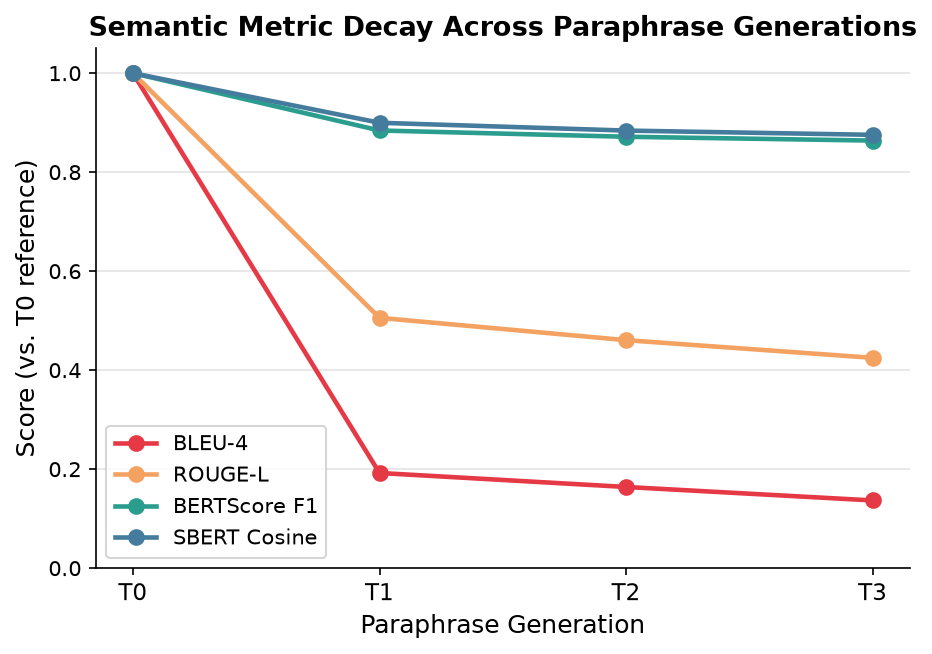
\includegraphics[width=0.95\columnwidth]{decay_curves/chatgpt/semantic_decay.png}
\caption{Similarity to T0 across generations for ChatGPT chains (700 docs). BLEU-4 and ROUGE-L
collapse at T1; BERTScore and SBERT retain most of their value.}
\label{fig:decay}
\end{figure}

\subsection{Paraphraser Comparison}

Table~\ref{tab:paraphrasers} compares all paraphrasers at T3.

\begin{table}[h]
\small
\centering
\caption{Similarity to T0 at T3 by paraphraser (700 docs), sorted by SBERT. Last column: share of
the T0$\to$T3 SBERT loss already incurred at T1.}
\label{tab:paraphrasers}
\resizebox{\columnwidth}{!}{%
\begin{tabular}{lccccr}
\toprule
\textbf{Paraphraser} & \textbf{BLEU-4} & \textbf{ROUGE-L} & \textbf{BERTSc.\ (resc.)} & \textbf{SBERT} & \textbf{@T1} \\
\midrule
Pegasus (slight)        & 0.643 & 0.810 & 0.830 & 0.925 & 41\% \\
DIPPER (low)            & 0.306 & 0.561 & 0.716 & 0.889 & 60\% \\
PaLM2                   & 0.277 & 0.541 & 0.659 & 0.876 & 80\% \\
ChatGPT                 & 0.137 & 0.425 & 0.592 & 0.875 & 80\% \\
Pegasus (full)          & 0.237 & 0.530 & 0.609 & 0.820 & 67\% \\
WordNet (rule-based)    & 0.400 & 0.756 & 0.698 & 0.785 & 37\% \\
DIPPER                  & 0.058 & 0.247 & 0.461 & 0.724 & 64\% \\
DIPPER (high)$^\dagger$ & 0.003 & 0.089 & 0.037 & 0.056 & -- \\
\bottomrule
\end{tabular}}
\\[2pt]{\footnotesize $^\dagger$Corpus artifact: outputs are largely unrelated to the source (Section~3.2).}
\end{table}

Figure~\ref{fig:trajectories} plots each paraphraser's path from T0 to T3 in the plane of
wording kept (BLEU-4) against meaning kept (SBERT). Every path starts at the original (1,1) and
runs far to the left but only slightly down: all paraphrasers sit well above the $y=x$ line, i.e.\
they discard wording much faster than meaning.

\begin{figure}[h]
\centering
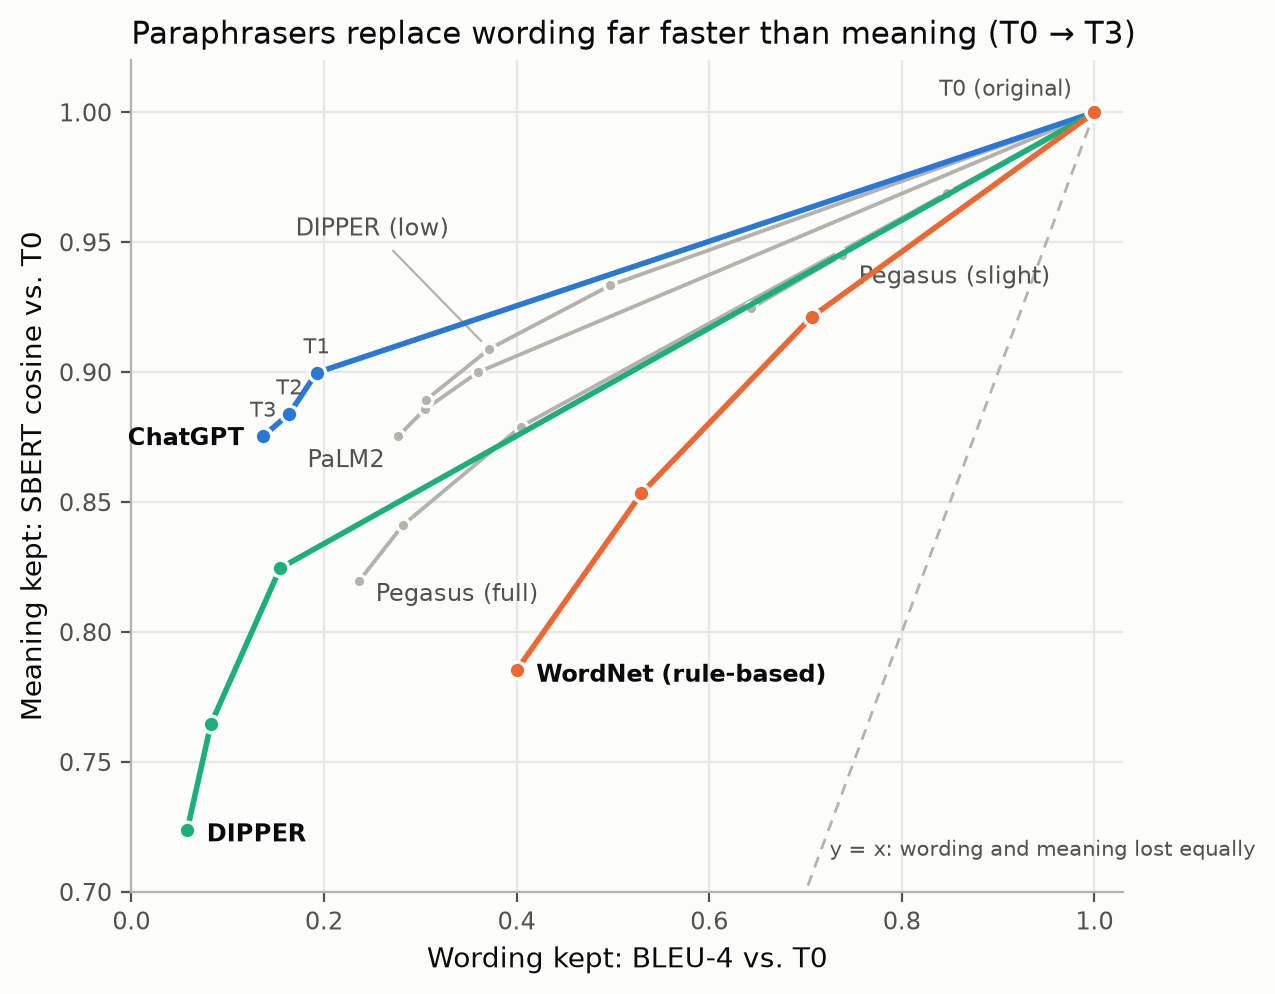
\includegraphics[width=\columnwidth]{decay_curves/paraphraser_trajectories.png}
\caption{Decay paths T0$\to$T3 per paraphraser (700 docs): wording kept (BLEU-4) vs.\ meaning kept
(SBERT), each relative to T0. ChatGPT moves almost straight left (wording replaced, meaning kept);
WordNet moves diagonally (meaning lost with wording); DIPPER loses most of both. DIPPER (high) is
omitted (unrelated outputs).}
\label{fig:trajectories}
\end{figure}

\textbf{The surface/meaning gap holds for every LLM paraphraser}, but its size varies. ChatGPT and
PaLM2 retain the same meaning (SBERT 0.875 vs.\ 0.876), yet ChatGPT keeps half of PaLM2's word
overlap (BLEU 0.137 vs.\ 0.277): it rewrites more aggressively at no semantic cost.
Conservative settings (Pegasus-slight, DIPPER-low) change least; default DIPPER removes the most
surface overlap (BLEU 0.058) and also loses the most meaning (SBERT 0.724).

\textbf{LLMs and the rule-based simulator decay in opposite ways.} WordNet keeps three times
ChatGPT's BLEU (0.400 vs.\ 0.137) yet loses more meaning by SBERT (0.785 vs.\ 0.875): synonym
substitution keeps the syntactic skeleton but breaks meaning, whereas an LLM rewrites the skeleton
and keeps the meaning. Rule-based simulation is therefore not a substitute for real LLM chains.
The two meaning metrics disagree here (rescaled BERTScore ranks WordNet above ChatGPT, 0.698 vs.\
0.592) because token-level matching rewards WordNet's preserved word order; SBERT compares the
whole-document meaning. We report both for this reason.

\textbf{Sharp vs.\ gradual loss depends on the paraphraser.} ChatGPT and PaLM2 incur 80\% of their
three-round SBERT loss at T1, whereas DIPPER (64\%), Pegasus-full (67\%) and WordNet (37\%) lose
meaning more gradually. This is a first semantic-level signal for \textbf{RQ2}'s question of
whether identity is lost sharply at T1; the attribution experiments will test it directly.

\textbf{DIPPER (high) is excluded from interpretation.} Its rescaled BERTScore (0.037) and SBERT
(0.056) are at the level of unrelated text, confirming the preprocessing check.

\subsection{Domain Comparison}

Table~\ref{tab:domain_metrics} reports SBERT at T3 by domain for four representative paraphrasers.

\begin{table}[h]
\small
\centering
\caption{SBERT similarity to T0 at T3 by domain (100 Human docs per domain).}
\label{tab:domain_metrics}
\resizebox{\columnwidth}{!}{%
\begin{tabular}{lcccc}
\toprule
\textbf{Domain} & \textbf{ChatGPT} & \textbf{PaLM2} & \textbf{DIPPER (low)} & \textbf{Pegasus (full)} \\
\midrule
Science (SciGen) & 0.947 & 0.969 & 0.925 & 0.857 \\
Summary (TLDR)   & 0.924 & 0.944 & 0.906 & 0.813 \\
News (XSUM)      & 0.888 & 0.912 & 0.870 & 0.787 \\
Review (Yelp)    & 0.854 & 0.859 & 0.887 & 0.831 \\
QA (ELI5)        & 0.850 & 0.828 & 0.867 & 0.827 \\
Opinion (CMV)    & 0.848 & 0.808 & 0.906 & 0.822 \\
Story (WP)       & 0.817 & 0.810 & 0.863 & 0.801 \\
\bottomrule
\end{tabular}}
\end{table}

\textbf{Technical and factual text keeps the most meaning.} Science, summaries and news rank highest
for ChatGPT and PaLM2: dense terminology, named entities and numbers must be copied, which anchors
meaning. \textbf{Creative and argumentative text keeps the least}: stories and opinions give the
paraphraser freedom to restructure narrative and rhetoric. Long documents in these domains are
also partly outside the SBERT window, which may contribute.
\textbf{Domain interacts with the paraphraser.} PaLM2 is the most domain-sensitive: it copies
heavily in science and news (BLEU 0.50 and 0.42) but almost fully rewrites opinion text (BLEU
0.11), while DIPPER (low) is nearly flat across domains. Domain will therefore be modelled jointly
with the paraphraser in later experiments.

\subsection{Stylometric Feature Evolution}

Table~\ref{tab:features} and Figure~\ref{fig:features} track stylometric features for ChatGPT.

\begin{table}[h]
\small
\centering
\caption{Stylometric features across ChatGPT generations (700 Human docs).}
\label{tab:features}
\begin{tabular}{lcccc}
\toprule
\textbf{Feature} & \textbf{T0} & \textbf{T1} & \textbf{T2} & \textbf{T3} \\
\midrule
Type--Token Ratio          & 0.629 & 0.670 & 0.678 & 0.682 \\
Function-Word Ratio        & 0.463 & 0.439 & 0.432 & 0.428 \\
Avg.\ Sentence Length      & 18.44 & 18.50 & 18.65 & 18.55 \\
Punct.\ Density (per 100w) & 16.77 & 15.70 & 15.46 & 15.41 \\
Avg.\ Word Length          & 4.679 & 5.106 & 5.165 & 5.215 \\
Avg.\ Doc.\ Length (words) & 248.8 & 195.1 & 188.4 & 183.8 \\
\bottomrule
\end{tabular}
\end{table}

\textbf{ChatGPT shortens and formalises.} Documents lose 22\% of their length at T1 and 26\% by T3.
Average word length rises sharply (4.68 $\to$ 5.22 characters) while the function-word ratio
(0.463 $\to$ 0.428) and punctuation density (16.8 $\to$ 15.4) fall: everyday words are replaced by
longer, more formal vocabulary. TTR rises (0.629 $\to$ 0.682); because TTR increases mechanically as
documents get shorter, we also measure the length-robust MATTR (50-word window), which rises too
(0.808 $\to$ 0.833, paired Cohen's $d_z = 0.61$): ChatGPT genuinely diversifies vocabulary.
Mean sentence length is stable ($\approx$18.5 words), but its per-document spread falls
(standard deviation 8.3 $\to$ 6.1 words, $d_z=-0.61$): sentence rhythm becomes more uniform.
As with the similarity metrics, most change happens at T1.

\textbf{Each paraphraser pushes style in its own direction.} At T3, DIPPER moves opposite to
ChatGPT: function-word ratio rises (0.463 $\to$ 0.527) and word length falls (4.68 $\to$ 4.41).
Pegasus-full splits sentences (18.4 $\to$ 11.9 words) and raises punctuation density
(16.8 $\to$ 18.1). PaLM2 stays close to the human values (function-word ratio 0.470, word length
4.82). These consistent, paraphraser-specific shifts are a first sign of the recoverable
``wood grain'' targeted by \textbf{RQ3}.

Figure~\ref{fig:scatter} places each ChatGPT generation by semantic retention (SBERT) and lexical
change (TTR), both relative to T0: the largest move happens between T0 and T1, after which
both quantities change little, mirroring the convergence seen in Table~\ref{tab:semantic_metrics}.

\begin{figure}[h]
\centering
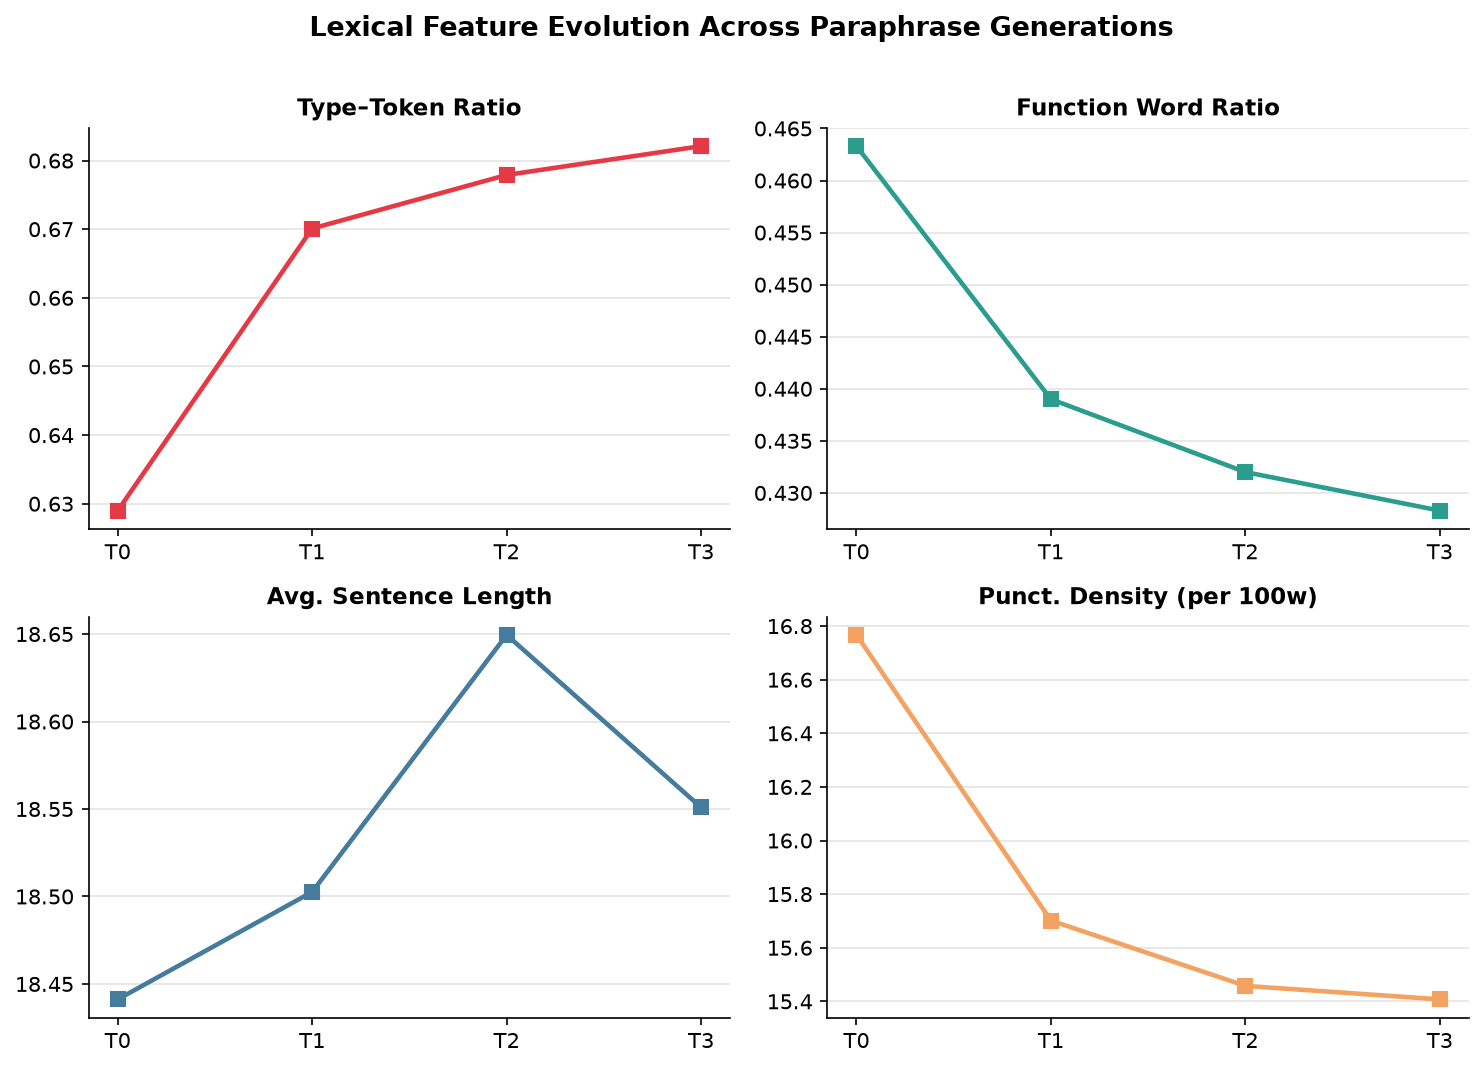
\includegraphics[width=0.95\columnwidth]{decay_curves/chatgpt/feature_evolution.png}
\caption{Stylometric feature evolution across T0--T3 for ChatGPT (700 docs). Word length rises and
function-word ratio falls; sentence length is stable.}
\label{fig:features}
\end{figure}

\begin{figure}[h]
\centering
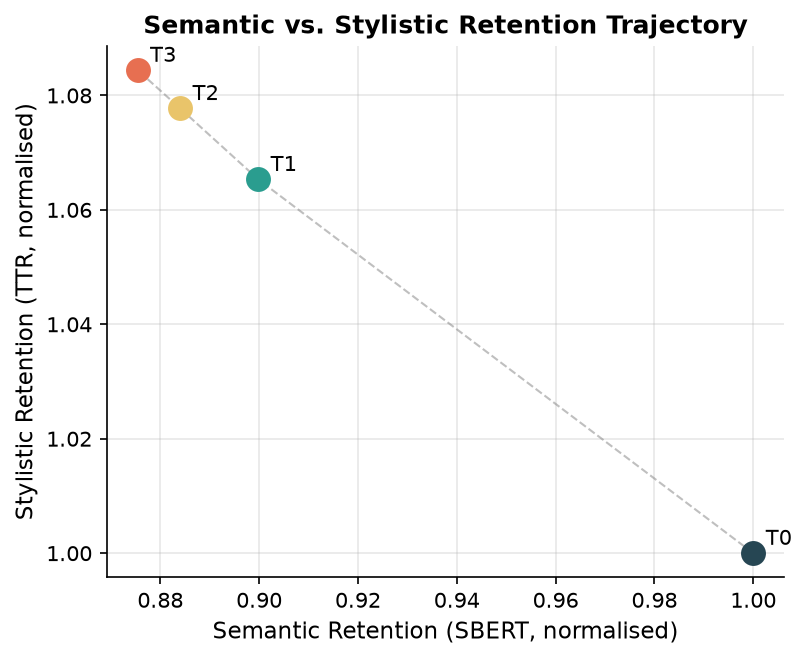
\includegraphics[width=0.95\columnwidth]{decay_curves/chatgpt/semantic_vs_stylistic.png}
\caption{Semantic retention (SBERT) vs.\ stylistic change (TTR), both normalised to T0, across
ChatGPT generations.}
\label{fig:scatter}
\end{figure}

\subsection{RQ1: Which Planks Are Replaced First?}
\label{sec:rq1}

Corpus averages can hide change: a feature can keep its mean while every document moves. For
RQ1 we therefore compare each document with \emph{its own} T0, separately for ten feature
families (``planks''), all computed from one spaCy parse (\texttt{en\_core\_web\_sm}):

\begin{itemize}[noitemsep,topsep=2pt]
  \item \emph{Lexical (skin):} word choice (Jaccard distance of word sets), function-word profile
        (relative frequencies of 198 function words), punctuation profile (12 marks), lexical
        richness (MATTR, average word length).
  \item \emph{Syntactic (skeleton):} sentence shape (mean and standard deviation of sentence
        length), Universal POS distribution, dependency-label distribution, tree depth (mean and
        maximum sentence depth, mean dependency distance), readability (Flesch--Kincaid grade).
  \item \emph{Meaning:} SBERT embedding (cosine distance).
\end{itemize}
Distributions are compared with the Jensen--Shannon distance and scalar features with the
root-mean-square difference of $z$-scores (standardised over all T0 documents).

\noindent\textbf{A common scale.} Raw distances of different families are not comparable, so each
is divided by the distance between the document's T0 and five \emph{unrelated} T0 documents of the
same domain: $\mathit{nd} = d(\mathrm{T}k, \mathrm{T0}) / d(\mathrm{T0}', \mathrm{T0})$. Retention
$R = 1 - \overline{\mathit{nd}}$ is 1 when the family is unchanged and 0 when the paraphrase is as
different from its source as another author's document is; $R<0$ means the paraphraser pushes the
text \emph{beyond} that, towards a style of its own. We report 95\% bootstrap confidence intervals
(1{,}000 resamples), paired one-sided Wilcoxon tests of $\mathit{nd}_{\text{style}} >
\mathit{nd}_{\text{meaning}}$ and of $\mathit{nd}(\mathrm{T}k{+}1) > \mathit{nd}(\mathrm{T}k)$ with
Holm correction, and rank-biserial effect sizes.

\begin{figure}[h]
\centering
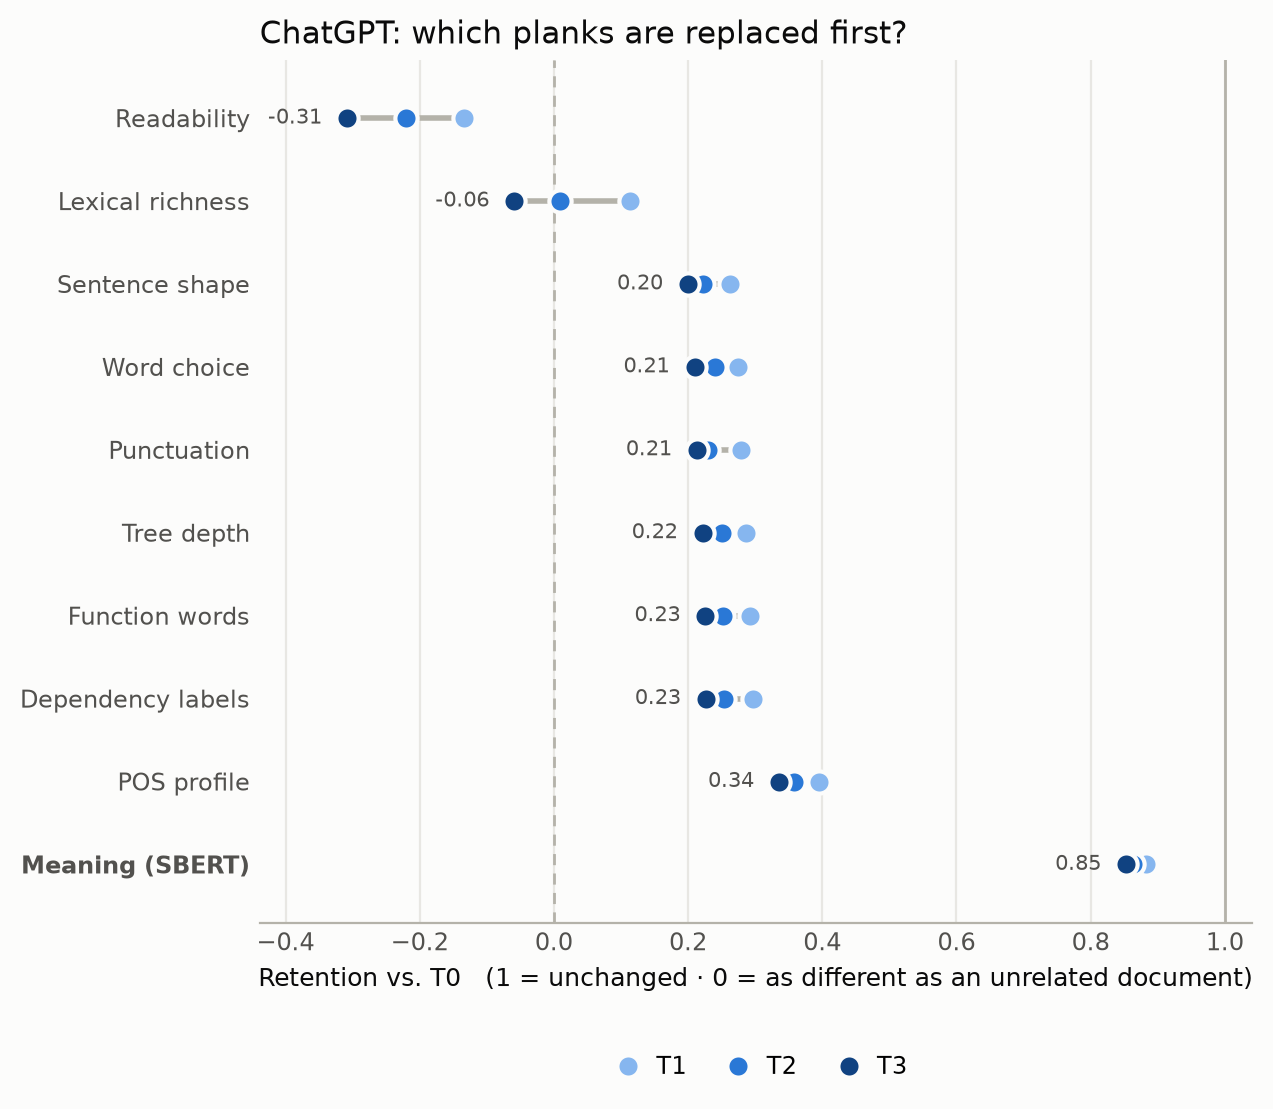
\includegraphics[width=\columnwidth]{decay_curves/chatgpt/linguistic_delta.png}
\caption{Retention of each feature family vs.\ T0 for ChatGPT chains (700 docs), sorted with the
first-replaced family on top. Every style family has lost most of its signal at T1; meaning keeps
0.85 at T3. Readability and lexical richness fall below 0: ChatGPT moves them further than the
gap between two human authors.}
\label{fig:delta}
\end{figure}

\begin{figure*}[t]
\centering
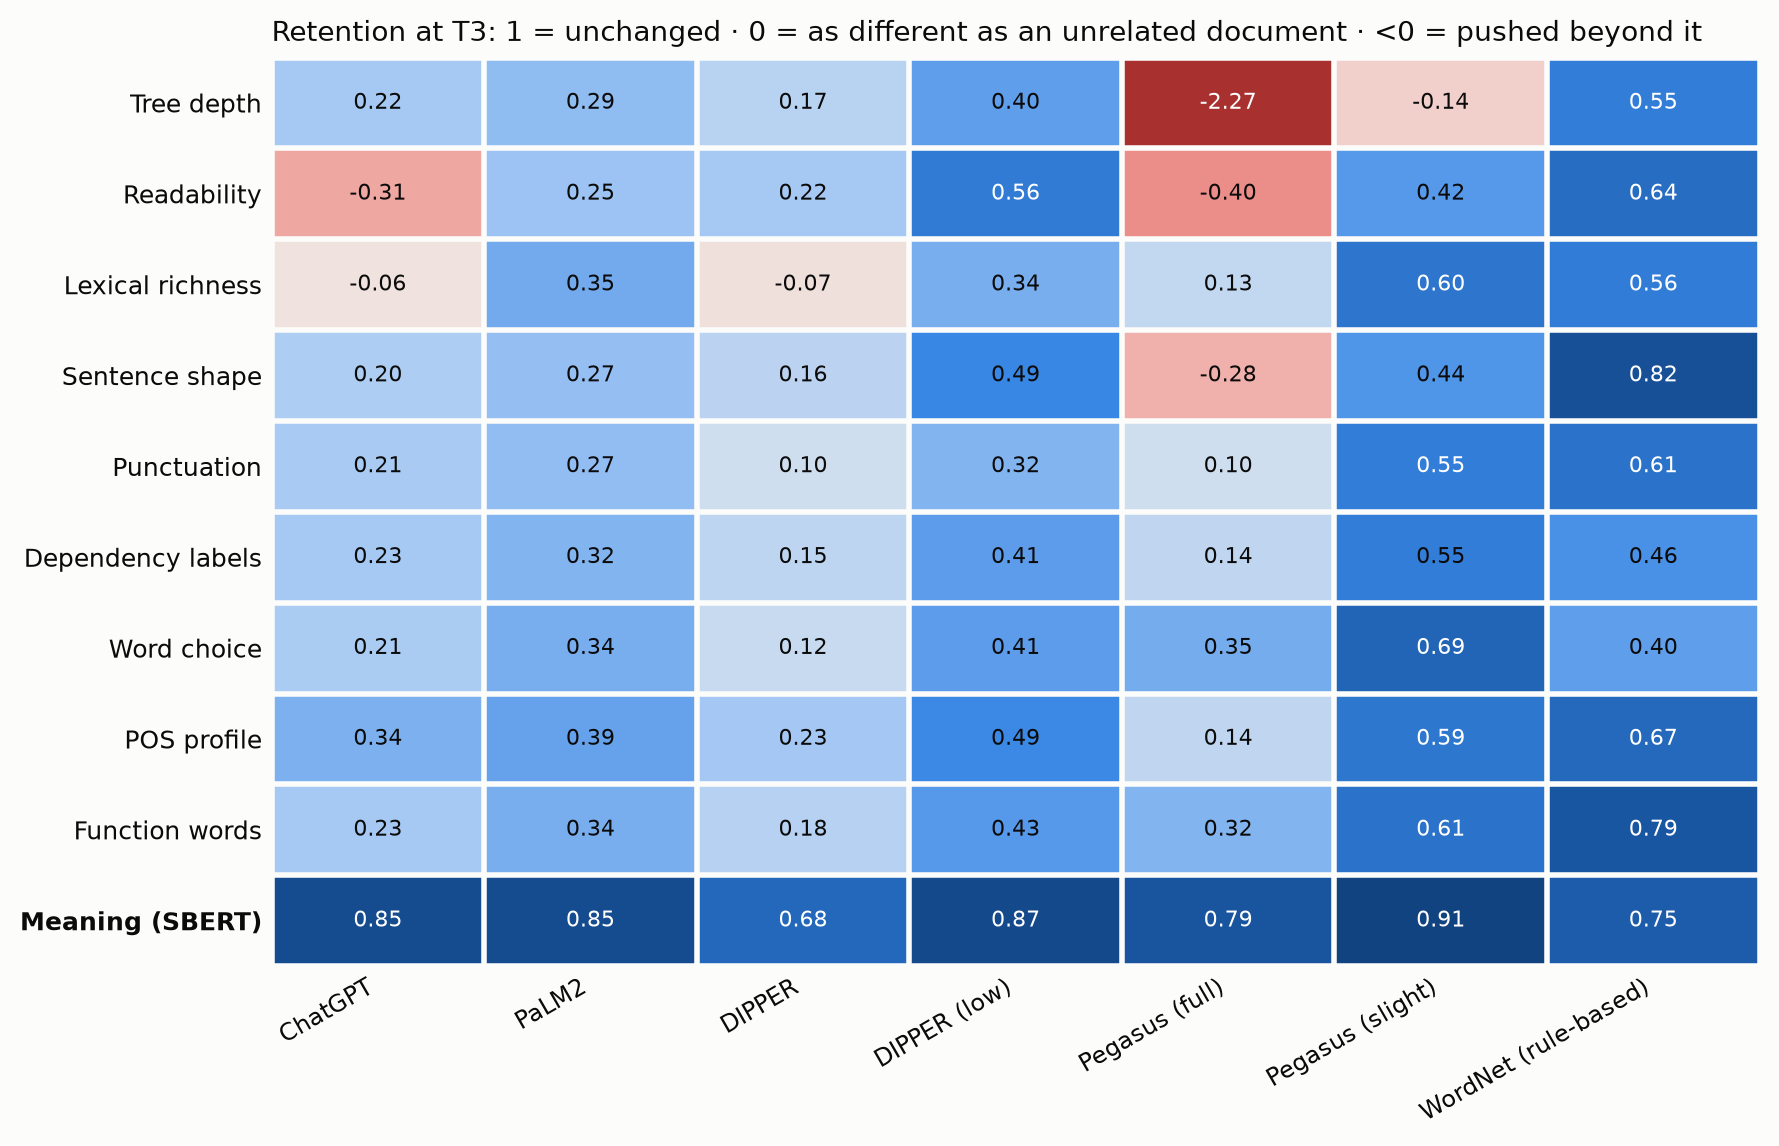
\includegraphics[width=0.85\textwidth]{decay_curves/retention_heatmap.png}
\caption{Retention at T3 for every feature family and paraphraser (DIPPER-high excluded).
Blue: share of the original signal kept; red: pushed beyond an unrelated document. Meaning (bottom
row) is the most retained family for every LLM paraphraser.}
\label{fig:retention}
\end{figure*}

\noindent\textbf{Style goes, meaning stays.} For ChatGPT (Figure~\ref{fig:delta}) every style
family retains 0.20--0.34 at T3, or less, while meaning retains 0.85 (95\% CI 0.85--0.86). The
pattern holds for every LLM paraphraser (Figure~\ref{fig:retention}): meaning is always the most
retained family, and in 61 of 63 paraphraser $\times$ family tests at T1 the style distance is
significantly larger than the meaning distance (Holm $p<0.05$). The two exceptions are both
WordNet (function words and sentence shape), whose word-for-word substitution leaves function
words and sentence boundaries in place while damaging meaning; it is the only paraphraser for
which some style families outlast meaning.

\noindent\textbf{The skeleton goes with the skin.} Syntactic families are \emph{not} more durable
than lexical ones for LLM paraphrasers. Mean retention at T3 (lexical vs.\ syntactic): ChatGPT 0.15
vs.\ 0.14, PaLM2 0.33 vs.\ 0.30, DIPPER 0.08 vs.\ 0.19. Pegasus-full restructures most aggressively
(syntactic $-0.53$): it splits sentences (18.3 $\to$ 12.7 words, $d_z=-1.04$), flattens parse trees
(depth 5.2 $\to$ 4.0, $d_z=-1.36$) and lowers the reading grade (9.8 $\to$ 6.6). Among style
families the POS profile is the most durable for ChatGPT, PaLM2 and DIPPER.

\noindent\textbf{Most planks are replaced in the first pass.} For ChatGPT and PaLM2, 82--92\% of each
style family's three-round loss occurs at T1; DIPPER 72--86\%; conservative settings and WordNet
spread it out (Pegasus-slight 41--57\%, WordNet 43--87\%). Later passes still change every family
significantly (Holm $p<0.05$ in 99\% of T1$\to$T2 and 100\% of T2$\to$T3 tests), but by small
amounts (ChatGPT median $\Delta\mathit{nd}$ 0.00--0.08).

\noindent\textbf{Paraphrasers replace style with their own.} Negative retention marks a systematic,
same-direction shift. ChatGPT raises the reading grade (9.8 $\to$ 12.4, $d_z=1.05$) and word length
(4.68 $\to$ 5.21, $d_z=1.50$) and uses fewer pronouns (0.079 $\to$ 0.064 of tokens, $d_z=-0.53$);
DIPPER does the opposite on word length (4.68 $\to$ 4.42) and lexical richness (MATTR 0.81 $\to$
0.77) and adds determiners (0.083 $\to$ 0.105, $d_z=0.70$). The direction of change identifies the
paraphraser, which motivates RQ3.

\noindent\textbf{Domains.} For ChatGPT, meaning retention at T3 ranges from 0.77 (stories) to 0.94
(science), and mean style retention from $-0.10$ (opinion) to 0.35 (science): technical text keeps
more of both, argumentative and narrative text the least.

\noindent\textbf{Preliminary answer to RQ1.} Under LLM paraphrasing, \emph{style is replaced long
before meaning}: after a single pass of ChatGPT, PaLM2 or DIPPER the style families have moved
55--90\% of the way to an unrelated author's style (some beyond it), while 79--88\% of the meaning
is retained; the syntactic
skeleton is replaced about as fast as the lexical skin, and several features are not just erased
but overwritten with a paraphraser-specific style.

\subsection{Limitations of the Current Analysis}

Results cover Human-authored T0 only; LLM-authored originals are processed but not yet analysed.
SBERT and BERTScore see only the first 256/512 subword tokens of long documents. DIPPER (high)
chains are unusable as released. Distribution features (function words, punctuation, POS,
dependencies) are noisier for short texts, and paraphrases are shorter than their sources, which
can inflate their distances; syntactic features rely on a small parser that may err more on
paraphrased text; Flesch--Kincaid uses a heuristic syllable count. The unrelated-document baseline
uses five partners per document from the same domain, so retention is relative to within-domain
variation.

%% ─────────────────────────────────────────────────────────────────────────────
\section{Plan for Next Steps}
%% ─────────────────────────────────────────────────────────────────────────────

\noindent\textbf{Limitations to address.} (i) Only Human-written T0 has been analysed; the six
LLM sources are preprocessed and will be compared next, including whether a model changes its
own text less (OpenAI T0 under ChatGPT, PaLM T0 under PaLM2). (ii) Paraphrases are shorter than
their sources and short texts give noisier profiles, so we will add a length-matched baseline.
(iii) SBERT reads only 256 tokens, which truncates 43\% of documents; a chunked encoding is
implemented, and a first check raises SBERT at T3 by 0.01--0.05 in long-text domains (ChatGPT on
stories: 0.817$\to$0.861), so final results will use it.

\noindent\textbf{Weeks 9--11: Authorship attribution (RQ2).} Train a stylometric SVM and a
fine-tuned RoBERTa to identify the seven sources on the train files, evaluate them on T0--T3, and
locate the ``point of no return'' per paraphraser.

\noindent\textbf{Weeks 10--12: Paraphraser fingerprinting (RQ3).} Train a paraphraser classifier
on T1--T3 (excluding DIPPER-high) with a key-level split, and visualise identity trajectories with
t-SNE and quantitative cluster-separation measures.

\noindent\textbf{Weeks 13--14: Synthesis.} A Streamlit decay dashboard and the final paper.


%% ─────────────────────────────────────────────────────────────────────────────
\bibliographystyle{ACM-Reference-Format}
\bibliography{references}

\end{document}
